
\chapter{Overview of \prism}
\label{sec:overview}

%\ma{I think we need to refer to the Prism theory paper in this section. We are giving the intuition behind the protocol here, but it's important to state that the security properties have been formally proved.}

The selection of a main chain in a blockchain protocol can be viewed as electing a leader block among all the blocks at each level of the blocktree. In this light, the blocks in the longest chain protocol can be viewed as serving three distinct roles: they stand for election to be leaders;  they add transactions to the main chain; they vote for ancestor blocks through parent link relationships. The latency and throughput limitations of the longest chain protocol are due to the {\em coupling} of the roles carried by the blocks. \prism removes these limitations by factorizing the blocks into three types of blocks: proposer blocks, transaction blocks and voter blocks. (Figure \ref{fig:prism}). Each block mined by a miner is randomly sortitioned into one of the three types of blocks, and if it is a voter block, it will be further  sortitioned into one of the voter trees. (Mining is described in detail in \S\ref{sec:mining}).

The proposer blocktree anchors the \prism blockchain. 
Each proposer block contains a list of reference links to transaction blocks, which contains transactions, as well as a single reference to a parent proposer block.
Honest nodes mine proposer blocks on the longest chain in the proposer tree, but the longest chain does not determine the final confirmed sequence of proposer blocks, known as the  \emph{leader sequence}. 
We define the \emph{level} of a proposer block as its distance from the genesis proposer block, and the \emph{height} of the proposer tree as the maximum level that contains any proposer blocks. 
The leader sequence of proposer blocks contains one block at every level up to the height of the proposer tree, and is  determined by the \emph{voter chains}. 

%\gw{Voter tree (blocktree) or voter chain (blockchain)? Since unlike proposer tree, only voter longest chain will participate in voting.}

There are $m$ voter chains, where $m \gg 1$ is a fixed parameter chosen by the system designer. For example, we choose $m=1000$ in our experiments.  The $i$th voter chain is comprised of voter blocks that are mined on the longest chain of the $i$th voter trees. A voter block votes for a proposer block by containing a reference link to that proposer block, with the requirements that: 1) a vote is valid only if the voter block is in the longest chain of its voter tree; 2) each voter chain votes for one and only one proposer block at each level. The leader block at each level is the one which has the highest number of votes among all the proposer blocks at the same level (tie broken by hash of the proposer blocks.) The elected leader blocks then provide a unique ordering of the transaction blocks to form the final ledger. (Ledger formation is explained in detail in \S\ref{sec:confirmation}.)





%%The security of the system rests on the security of the $m$ voter chains, which is guaranteed by longest chain protocol. However, as we discuss next, by relying on many parallel voter chains, \prism significantly reduces the latency required to achieve a desired reversal probability compared to the vanilla longest chain protocol.


\if 0
The voter blocks vote for transactions indirectly by voting for proposer blocks, which in turn link to transaction blocks. Proposer blocks are grouped according to their level in the original block tree \ma{not clear what this means. what is the `original block tree'? does a proposer block have a link to a parent proposer block (this is not shown in the figure)}, and each voter tree votes for exactly one proposer block at each level to select a leader block among them. The leader block is the proposer block which has the highest number of votes among all the proposer blocks at the same level (ties broken by hash of the proposer blocks.) The elected leader blocks can then bring in the transactions to form the final ledger. \ma{Can we explain this more precisely, e.g., To obtain the final ledger, one traverses the elected leader blocks level by level, including the transactions that they link to in order.} The vote from a voter tree is represented by the reference link from a voter block in the longest chains of the voter tree; the longest chains in all the $m$ voter trees maintain the security of the whole system, as explained next.

\fi

%\begin{figure}
%    \centering
%    \tikzstyle{proposer} = [draw, fill=blue!20, rectangle, rounded corners, minimum height=1em, minimum width=1.6em, text centered]
\tikzstyle{voter} = [draw, fill=green!20, rectangle, rounded corners, minimum height=1em, minimum width=1.6em]
\tikzstyle{transaction} = [draw, circle, fill=yellow!20]

% The block diagram code is probably more verbose than necessary
\begin{tikzpicture}[auto, node distance=0.8cm,>=latex']
\node [proposer] (p0l) {\tiny L};
\node [proposer, below of=p0l] (p1l) {\tiny L};
\node [proposer, left=0.1cm of p1l] (p1s) {};
\node [proposer, below of=p1l] (p2l) {\tiny L};
\node [proposer, right=0.1cm of p2l] (p2s) {};
\node [proposer, below of=p2l] (p3l) {\tiny L};

\node[transaction, above left = 0.01cm and 0.45cm of p0l] (t00){};
\node[transaction, below right = 0.06cm and 0.02cm of t00] (t01){};
\node[transaction, left = 0.25cm of p1s] (t10){};
\node[transaction, above right = 0.07cm and 0.02cm of t10] (t11){};
\node[transaction, below right = 0.10cm and 0.07cm of t10] (t12){};
\node[transaction, below left = 0.05cm and 0.25cm of p2l] (t20){};
\node[transaction, above left = 0.07cm and 0.13cm of t20] (t21){};
\node[transaction, left = 0.35cm of p3l] (t30){};
\node[transaction, above left = 0.05cm and 0.11cm of t30] (t31){};
\node[transaction, left = 0.25cm of t30] (t32){};
\draw[densely dashed, <-] (t00)  to [looseness=0.4] (p0l);
\draw[densely dashed, <-] (t01)  to [looseness=0.4] (p0l);
\draw[densely dashed, <-] (t10)  to [looseness=0.4] (p1l);
\draw[densely dashed, <-] (t11)  to [looseness=0.4] (p1l);
\draw[densely dashed, <-] (t12)  to [looseness=0.4] (p1l);
\draw[densely dashed, <-] (t20)  to [looseness=0.4] (p2l);
\draw[densely dashed, <-] (t21)  to [looseness=0.4] (p2l);
\draw[densely dashed, <-] (t30)  to [looseness=0.4] (p3l);
\draw[densely dashed, <-] (t31)  to [looseness=0.4] (p3l);
\draw[densely dashed, <-] (t32)  to [looseness=0.4] (p3l);


\node [voter, right=1cm of p0l] (v00) {};
\node [voter, below of=v00] (v01) {};
\node [voter, below of=v01] (v02) {};
\node [voter, below of=v02] (v03) {};
\draw[<-] (v00) to (v01);
\draw[<-] (v01) to (v02);
\draw[<-] (v02) to (v03);

\node [voter, right=0.3cm of v00] (v10) {};
\node [voter, below of=v10] (v11) {};
\node [voter, below of=v11] (v12) {};
\node [voter, below of=v12] (v13) {};
\draw[<-] (v10) to (v11);
\draw[<-] (v11) to (v12);
\draw[<-] (v12) to (v13);

\node [right=0.3cm of v10] (space0) {$\cdots$};
\node [below of=space0] (space1) {$\cdots$};
\node [below of=space1] (space2) {$\cdots$};
\node [below of=space2] (space3) {$\cdots$};

\node [voter, right=0.3cm of space0] (v20) {};
\node [voter, below of=v20] (v21) {};
\node [voter, below of=v21] (v22) {};
\node [voter, below of=v22] (v23) {};
\draw[<-] (v20) to (v21);
\draw[<-] (v21) to (v22);
\draw[<-] (v22) to (v23);

\draw[densely dashed, <-] (p0l)  to [looseness=0.3] (v00);
\draw[densely dashed, <-] (p1l)  to [looseness=0.3] (v01);
\draw[densely dashed, <-] (p2l)  to [looseness=0.3] (v02);
\draw[densely dashed, <-] (p3l)  to [looseness=0.3] (v03);

\draw[densely dashed, <-] (p0l)  to [looseness=0.3] (v10);
\draw[densely dashed, <-] (p1l)  to [looseness=0.3] (v11);
\draw[densely dashed, <-] (p2l)  to [looseness=0.3] (v12);
\draw[densely dashed, <-] (p3l)  to [looseness=0.3] (v13);

\draw[densely dashed, <-] (p0l)  to [looseness=0.3] (v20);
\draw[densely dashed, <-] (p1l)  to [looseness=0.3] (v21);
\draw[densely dashed, <-] (p2l)  to [looseness=0.3] (v22);
\draw[densely dashed, <-] (p3l)  to [looseness=0.3] (v23);

\end{tikzpicture}
%    \caption{\prism: Factorizing the blocks into three types of blocks: proposer blocks, transaction blocks and voter blocks. \ma{can we increase the font size a bit?} }
%    \label{fig:prism}
%\end{figure}

\begin{figure}
\begin{center}
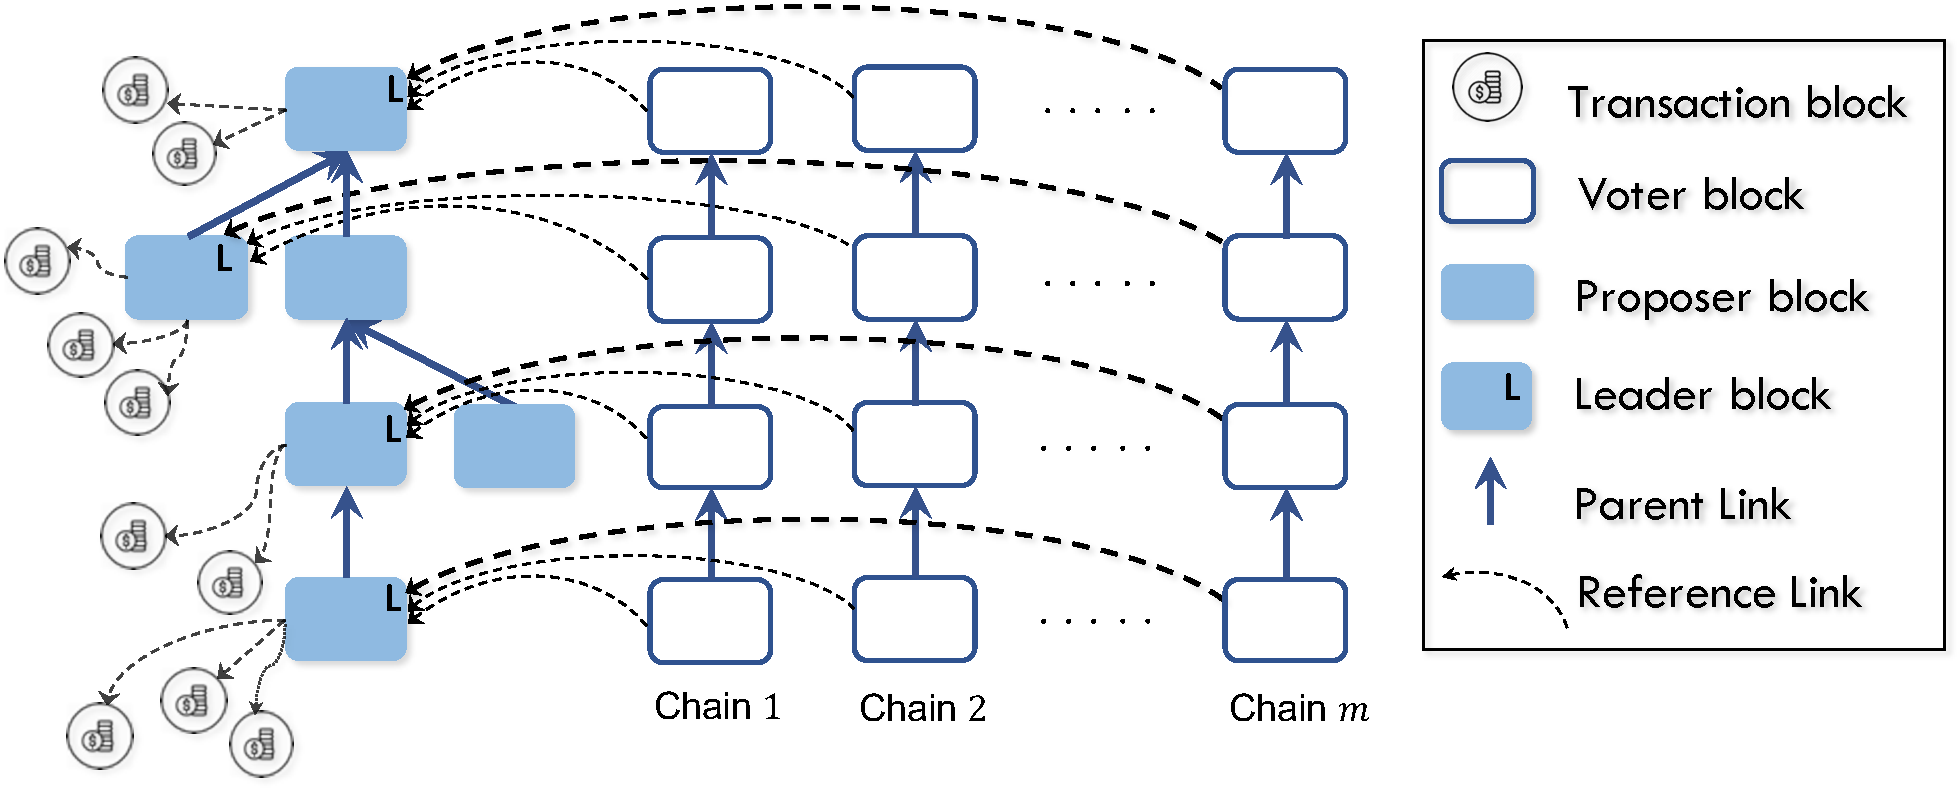
\includegraphics[width=0.45\textwidth]{figures/Prism_main.pdf}
\end{center}
\vspace{-2mm}
\caption{\small \prism: Factorizing the blocks into three types of blocks: proposer blocks, transaction blocks and voter blocks.}
\label{fig:prism}
\vspace{-5mm}
\end{figure}

%%Thus, the parent links in the original block tree have two implicit functionalities which are explicitly separated in this representation: 1) they provide a partial ordering of the proposal blocks according to their levels, and 2) they allow blocks to vote for each other. 
% they help the voting blocks to vote for each other.
%%\blue{It's unclear here what is meant by having a block ``support" another block.}

\if 0

\section{Security Model}
\vb{Let $\mathcal{N}$ denote  the nodes in the system and with of loss of generality, we assume each node has equal mining power. Let $\mathcal{H} \subseteq \mathcal{N}$ denote the set of honest nodes and $\mathcal{N} \setminus \mathcal{H}$ is set the adversarial nodes. The fraction of adversarial nodes, $\beta = 1 - \frac{|\mathcal{H}|}{|\mathcal{N}|}$, is assumed to be less then $0.5$. 
%We assume a network model where the delay for a block of size $B$ is equal to $\Delta = \frac{B}{C}+D$, where $B/C$ is the processing delay and $D$ is the propagation delay.
%We model the protocol as running in rounds where each round is of duration equal to the delay ($\Delta$) corresponding to the largest sized block in the \prism protocol. 
The adversarial nodes do not have to follow the \prism protocol - they can mine new blocks with any content and anywhere on the blockchain, and  unlike honest users, they can keep their mined block in private and release it anytime in future. 
%c) their action in a given round is a function of the action of the honest nodes up to and including that round.
However, the adversary cannot perform certain actions such as modifying the block content of blocks mined by honest nodes or withholding blocks mined by an honest node from reaching other honest nodes.
}

\fi

\section{Security and Latency}
\label{sec:prism-latency}

%The ledger is maintained by the leader proposer blocks at all the levels. 

The votes from the voter trees secure each leader proposer block, because changing an elected leader requires reversing enough votes to give them to a different proposer block in that level. 
Each vote is in turn secured by the longest chain protocol in its voter tree. If the adversary has less than $50\%$ hash power, and the mining rate in each of the voter trees is kept small to minimize forking,  then the consistency and liveness of each voter tree guarantee the consistency and liveness of the ledger maintained by the leader proposer blocks. 
However, this would appear to require a long latency to wait for each voter block to get sufficiently deep in its chain. What is interesting is that when there are many voter chains, the same guarantee can be achieved without requiring each and every vote to have a very low reversal probability, thus drastically improving over the latency of the longest chain protocol. 


To get some intuition, consider the natural analog of the private double-spend attack on the longest chain protocol in \prism. Figure \ref{fig:double_spend}(b) shows the scenario. An honest proposer block $Ho$ at a particular level has collected votes from the voter chains. Over time, each of these votes will become deeper in its voter chain. An attack by the adversary is to mine a private proposer block $A$ at the same level, and on each of the voter trees, fork off and mine a private alternate chain and send its vote to block $A$. After leader block $Ho$ is confirmed, the adversary continues to mine on each of the alternate voter chains to attempt to overtake the public longest chain and shift the vote from $Ho$ to $A$. If the adversary can thereby get more votes on $A$ than on $Ho$, then its attack is successful. The question is how deep do we have to wait for each vote to be in its voter chain in order to confirm the proposer block $Ho$?

Nakamoto's calculations will help us answer this question. As an example, at tolerable adversary power $\beta = 30\%$, the reversal probability in a single chain is $0.45$ when a block is $2$-deep \cite{bitcoin}. With $m=1000$ voter chains and each vote being $2$-deep, the expected number of chains that can be reversed by the adversary is $450$. The probability that the adversary can get lucky and reverse more than half the votes, i.e. $500$, is about  $0.001$. Hence to achieve a reversal probability, $\epsilon = 0.001$, we only need to wait for the votes to be  $2$-deep, as opposed to the $24$ block depth needed in the longest chain protocol (\S\ref{s:lc-latency}). This reduction in latency comes without sacrificing security: each voter chain can operate at a slow enough mining rate to tolerate $\beta$ adversarial hash power. Furthermore, increasing the number of voter chains can further improve the confirmation reliability without sacrificing latency; for example, doubling the number of voter chains from $1000$ to $2000$ can reduce the reversal probability from $0.001$ to $10^{-6}$.

We have discussed one specific attack, focusing on the case when there is a single public proposer block on a given level. Another possible attack is when there are two or more such proposer blocks and the adversary tries to balance the votes between them to delay confirmation. It turns out that the attack space is quite huge and these are formally analyzed in \cite{prism-theory} to obtain the following guarantee on the confirmation latency, regardless of the attack:

 \begin{theorem}[Latency, Thm. 4.8 \cite{prism-theory}] \label{cor:latency_fast}
For an adversary with $\beta< 50\%$ of hash power, network propagation delay $D$, \prism with $m$ chains confirms  \textit{honest}\footnote{Honest transactions are ones which have no conflicting double-spent transactions broadcast in public.} transactions at reversal probability $\epsilon$ guarantee with latency upper bounded by
\begin{equation}
\label{eq:latency}
 Dc_1(\beta) +  \frac{Dc_2(\beta)}{m} \log \frac{1}{\epsilon}\;\; \text{ seconds},
\end{equation}
where $c_1(\beta)$ and $c_2(\beta) $ are $\beta$ dependent constants.
\end{theorem}

For large number of voter chains $m$, the first term dominates the above equation and therefore Prism achieves near optimal latency, i.e. proportional to the propagation delay $D$ and independent of the reversal probability. Figure \ref{fig:rd} compares the latency-reliability tradeoffs of \prism and the longest chain protocol. Note that (\ref{eq:latency}) is a worst-case latency bound that holds for {\em all} attacks. In Section \ref{sec:balancing}, we will evaluate the latency of our system under the balancing attack. 


\section{Throughput}
\label{sec:thruput}

To keep \prism secure, the mining rate and the size of the voter blocks have to be chosen such that each voter chain has little forking. The mining rate and the size of the proposer blocks have to be also chosen such that there is very little forking in the proposer tree. Otherwise, the adversary can propose a block at each level, breaking the liveness of the system. Hence, the throughput of \prism would be as low as the longest chain protocol if transactions were carried by the proposer blocks directly. 


To decouple security from throughput, transactions are instead carried by separate transaction blocks. Each proposer block when it is mined refers to the transaction blocks that have not been referred to by previous proposer blocks. This design allows throughput to be increased by increasing the mining rate of the transaction blocks, without affecting the security of the system. The throughput is only limited by the computing or communication bandwidth limit $C$ of each node, thus potentially achieving $100\%$ utilization. In contrast, as we discussed in \S\ref{s:lc-thput}, the throughput of the longest chain protocol is security-limited, resulting in low network utilization. \cite{prism-theory} formally proves that \prism achieves near optimal throughput:

\begin{theorem}[Throughput, Thm. 4.4\cite{prism-theory} ]
\label{thm:throughput} For an adversary with $\beta < 50\%$ fraction of hash power and network capacity C, Prism can achieve  $(1-\beta)C$ throughput and maintain liveness in the ledger.
\end{theorem}

%Note that the reference links from a proposer block to its transaction blocks are sealed in the proof-of-work of the proposer block. Hence, once a proposer block is mined, there is no way for an attacker to change the reference links to the transaction blocks. In contrast, the transactions that a miner in \bitcoin-NG adds onto the ledger after its block enters the main chain are {\em not} sealed by the proof-of-work. Hence, \bitcoin-NG is susceptible to censorship attacks.

\smallskip
\noindent{\bf Remark on security model:} The Prism theory paper~\cite{prism-theory} analyzed the protocol in a synchronous round-based network model under standard assumptions about the adversary. In particular, the delay for a block of size $B$ was assumed to be equal to $\Delta = \frac{B}{C}+D$, where $B/C$ is the processing delay and $D$ is the propagation delay, and the protocol was assumed to run in rounds where each round is of duration equal to the delay ($\Delta$) corresponding to the largest sized block. The adversarial nodes do not have to follow protocol - they can mine new blocks with any content and anywhere on the blockchain, and  unlike honest users, they can keep their mined blocks in private and release them at anytime in the future. However, the adversary cannot modify the content of blocks mined by honest nodes or withhold blocks mined by an honest node from reaching other honest nodes. Refer to \S2 of~\cite{prism-theory} for the full specification of the model. This model does not capture the impact of artifacts like queuing delay or asynchronous communication on performance. Nevertheless our implementation shows that the overall performance characteristics predicted by the theory hold in a practical setting. 


% To decouple security from throughput, transactions are instead carried by separate transaction blocks. The transaction blocks enter into a pool after they are mined. Each proposer block when it is mined refers to the transaction blocks in the pool that have not been referred to by previous proposer blocks. When a proposer block is confirmed to be the leader of its level, the transactions in all the transaction blocks it refers to enter into the ledger. \ma{The last three sentences could be cut from here and discussed in the design section} The throughput of the system can be increased by increasing the mining rate of the transaction blocks, without affecting the security of the system. This throughput is only limited by the computing or communication bandwidth limit $C$ of each node, thus potentially achieving $100\%$ utilization. In contrast, as we discussed in \S\ref{s:lc-thput}, the throughput of the longest chain protocol is security-limited, resulting in low network utilization. 





%\ma{If we include the figure I mentioned at the end of 2.1, which shows the relationship between $f\Delta$ and security, then we can recall that in the section and explain that transaction blocks overcome this problem}


%%Show that Prism is the optimal (theory). See Fig.~\ref{fig:protocols-comparison}. Optimal in terms of communication limit. But the implementation is limited by state execution. Compare to Hotstuff. 



% \subsection{Formal guarantees}
% The results established about the \prism protocol in a recent theoretical paper~\cite{prism-theory} provide the following throughput and latency guarantees. \ly{update the bib file to reflect that the paper has been published. also consider anonymous issues}




% The above two results show that of Prism achieves near optimal throughput and latency.

% \ma{@Vivek: please summarize the main results from the theory paper here.}
% \vb{done.}



\if 0

\begin{figure}
\begin{center}
\includegraphics[width=0.4\textwidth]{chains-table.jpg}
\end{center}
\caption{\label{fig:protocols-comparison} Table: Comparison }
\end{figure}

\fi
